\documentclass{article}
\usepackage[utf8]{inputenc}
\usepackage[danish]{babel}

\usepackage{ragged2e}
\usepackage[labelfont=bf, font={small,it}]{caption}
\usepackage{graphicx}
\usepackage{float}
\usepackage[
    colorlinks=true,
    pdfborder={0 0 0},
    linkcolor=blue,
    citecolor=magenta
]{hyperref}

\graphicspath{ {images/} }

\title{Microservices og Availability}
\author{Adam Lass og Rasmus Helsgaun}
\date{18. december 2020}

\begin{document}

\maketitle
\begin{flushleft}
\subsection*{Abstract}
Ensuring high availability in a monolithic application is almost impossible due to its deployment and scalability challenges. This poses a big threat to businesses with a monolithic system today, that want to scale tomorrow. In this article we will explore how Microservices attempts to solve these challenges, and at what cost. By implementing this architecture when appropriate, businesses stand to win big on flexibility, scalability and availability of their systems.

\section*{Hvad indebærer availability?}
Når der er tale om availability, refereres der til tilgængeligheden af software og dets evne til at udføre en opgave, når der er brug for det. Konceptet bygger på reliability, som handler om hvor pålidelig et system er, og inkorporerer tilmed også konceptet om gendannelse af systemet ved fejl. I denne artikel vil der blive set nærmere på, hvordan Microservices kan skabe værdi for en kunde i form af availability, og hvilken bekostning det har sammenlignet med en monolitisk arkitektur.

\section*{Hvad er en monolitisk arkitektur?}
Den monolitiske arkitektur beskriver en softwareapplikation, hvortil alle komponenter er samlet i et enkelt system. \linebreak

\begin{figure}[H]
    \captionsetup{justification=raggedright,singlelinecheck=false}
    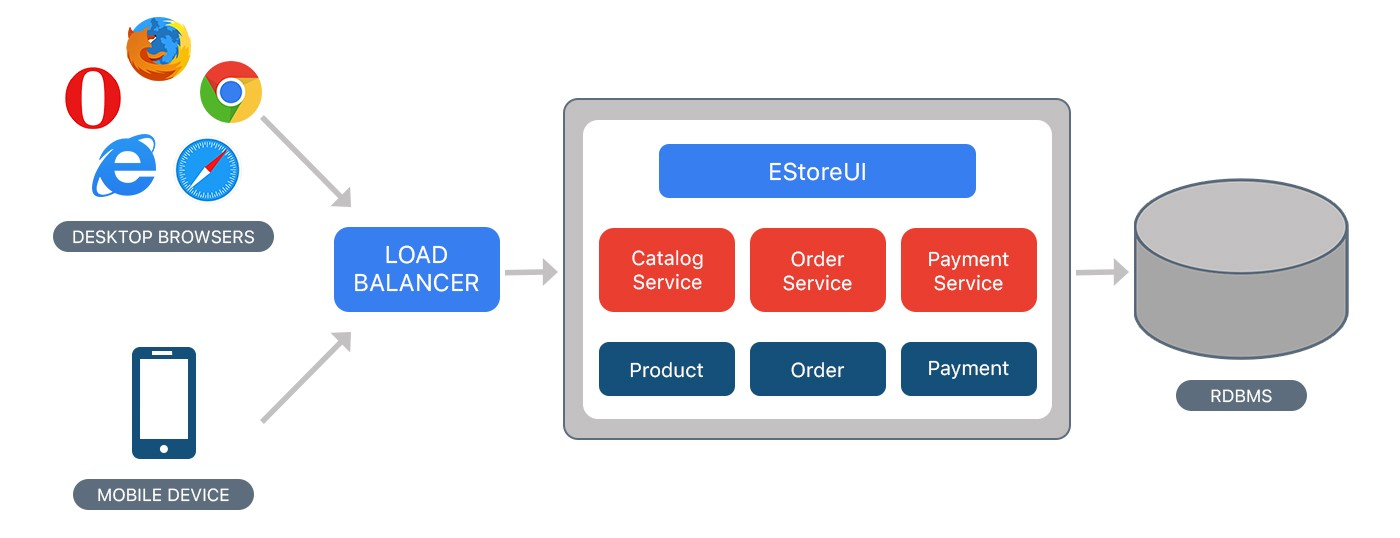
\includegraphics[width=\textwidth]{monolithic load balance.jpeg}
    \caption{Illustrerer opsætningen af den monolitiske arkitektur, med alle systemets komponenter samlet i ét modul bagved en load balancer.\cite{mono2} \label{figure:mono load balance}}
\end{figure}

Fordelene ved at bruge en monolitisk arkitektur er blandt andet, at det i de tidlige stadier kan være enkelt at udvikle, deploye og teste, da man har alle komponenter samlet i én applikation.\cite{mono1} Givet at ens monolitiske system er udviklet stateless, er det også forholdsvist simpelt at skalere horisontalt, ved at køre flere instanser af systemet bag en load balancer, som illustreret på \textbf{figur 1}.\cite{mono2} \linebreak

Der er dog også en række ulemper ved at udvikle og vedligeholde et monolitisk system, som bør overvejes inden den vælges som arkitektur. Eksempelvis kan det være sværere at vedligeholde et monolitisk system, da størrelsen af komponenterne, og afhængighederne derimellem, kan øge systemets kompleksitet. Den øgede kompleksitet medfører ofte en høj kobling, hvilket forværrer fleksibiliteten og overskueligheden af systemet.\cite{mono3} Dette kan have store negative implikationer for udefrakommende udvikleres forståelse og overblik af systemet, hvilket kan resultere i øgede tidsmæssige og økonomiske udgifter ved videreudvikling.\cite{mono4} \linebreak

Samtidigt kan størrelsen have betydning for en længere opstartstid, hvilket er essentielt at holde til et minimum under opdateringer eller efter, at systemet er crashet. I sådanne tilfælde bærer arkitekturen i særdeleshed præg af, at en lille opdatering eller crash af et komponent kræver et fuldt genstart af alle komponenterne.\cite{mono5} Hvis ikke disse scenarier bliver håndteret ordentligt, kan det resultere i at arkitekturen har en stor negativ indflydelse på reliability og availability af applikationen. En måde at håndtere et crash på kan være ved at bruge horisontal skalering. Her kan services, der stadig kører, overtage trafikken for services der er i fejltilstand eller under genopretning. Tilmed kan et værktøj oven på dette, såsom Kubernetes’ Rolling Updates\cite{micro2}, hjælpe med at bevare et systems availability under opdateringer. 

\section*{Hvad er Microservices?}
Microservices er en arkitektonisk stil der samler services, der specialiserer sig i forskellige egenskaber, som tilsammen udgør en større applikation. Dette er et direkte modstykke til den monolitiske arkitektur, hvor alle egenskaber ligger i samme service.\linebreak

\begin{figure}[H]
    \captionsetup{justification=raggedright,singlelinecheck=false}
    \includegraphics[width=\textwidth]{monolithic and Microservices.jpg}
    \caption{Illustrerer forskellen mellem den Monolitiske arkitektur og Microservices arkitekturen.\cite{micro8}  \label{figure:mono micro}}
\end{figure}
Den opdelte arkitektur set i \textbf{figur 2} bringer en række fordele til områder af udviklingen i form af availability, scalability, testability, deployment m.fl., men har samtidigt også en række ulemper med sig.\cite{mono2} En meget dominerende fordel ift. availability er eksempelvis, hvordan Microservices gerne skal være små og afgrænset i forhold til deres egenskaber.\cite{micro1} Dette har nemlig den betydning, at potentiel downtime på den enkelte service, bliver mindre alvorlig, da den nu kun eksisterer som en mindre del af et større system. Sådan en downtime kan være forårsaget af bugs der får servicen til at crashe, men også af almindelige opdateringer af servicen, begge ting som er forventelige i dagligdagen. Størrelsen af en Microservice bringer også den fordel, at man kan skalere de enkelte services horisontalt ud fra behov. Dette kan have en positiv indflydelse på ens hosting omkostninger og opstartstid, da man kan undgå unødvendig skalering af ressourcer.\cite{micro9} \linebreak

Det er dog også værd at nævne, at man ved brug af den alternative Nanoservices arkitektur\cite{nano}, via frameworks såsom serverless\cite{serverless}, yderligere kan optimere skaleringen ved at gøre den dynamisk ud fra det aktuelle behov af de enkelte funktioner. Skal ens applikation kunne håndtere meget varierende trakfik, kan man derfor med brug af Nanoservices opnå en endnu mere agil skaleringsmodel, der både øger availability og reducerer de gennemsnitlige hosting omkostninger.\cite{micro3} Her er det dog vigtigt at nævne det overhead, der ligger i at funktionerne, kun bliver brugt én gang, hvilket også har en negativ effekt på responstiden. Dette betyder også, at der samtidigt skal være nok variation i trafikken, før man kan opnå de økonomiske besparelser, når man benytter sig af en Nanoservices arkitektur.\linebreak

En betydelig fordel som Microservices bringer er dets testability. Selvstændigheden og isolationen af komponenterne gør det nemmere at skrive tests, da afhængighederne imellem komponenterne er mindre sammenlignet med et monolitisk system.\cite{micro4} Givet det faktum, at tests skaber bedre kode, der sjældnere fejler\cite{micro5}, kan man udlede, at bedre testability, i overført betydning, også skaber bedre availability.\linebreak

I det store hele kan brugen af Microservices være fordelagtig i forhold til availability, men der ligger selvfølgelig også en række udfordringer forbundet med at implementere arkitekturen. Udviklingsmæssigt skal man som udvikler ofte bruge meget tid på, at hver enkelt komponent kan stå alene. Dette indebærer ofte ting som authentication, authorization, logging, osv., alle ting som man i et monolitisk system kun skal implementere én gang.\cite{micro6} En anden udfordring er, at de forskellige komponenter ofte skal snakke med hinanden via protokoller såsom HTTP, hvilket tilføjer ekstra netværkstrafik og processering i eventuelt implementerede loadbalancers. Dette kan både resultere i længere svartider og større regninger hos cloud leverandøren, begge ting man gerne vil forsøge at undgå, især som en mindre virksomhed.\cite{micro7}

\section*{Overgangen til Microservices}
Trods de ovenstående udfordringer viser en undersøgelse udført af O'Reilly\cite{oreilly} i 2020, med 1502 deltagere\cite{research}, at 61\% allerede har brugt Microservices i et år eller mere. I en anden undersøgelse lavet af Bernd Ruecker i 2018, med 354 deltagende virksomheder\cite{research2}, ses det at der trods den ekstra udviklingbyrde ved Microservices, alligevel er en interesse i at bruge arkitekturen til at opnå hurtigere udviklingstid hos 60\% af deltagerne. Dette er nok i høj grad præget af den ekstra fleksibilitet Microservices giver, når der skal integreres med eksisterende systemer i de større virksomheder. Tilmed beskriver en artikel\cite{mono3}, udgivet hos Divante\cite{divante}, hvordan store tech giganter såsom Amazon, Netflix og Spotify startede ud med en monolitisk arkitektur, og siden hen har gået over til at bruge Microservices.

\section*{Konklusion}
Det ses, at den generelle udvikling i valg af arkitektur, både i større og mindre virksomheder, går i retningen mod at bruge Microservices. Dette skyldes i høj grad, at arkitekturen er bedre egnet til, at håndtere de udfordringer, der kommer med at bygge store systemer, som skal kunne håndtere meget brugertrafik. Valget kommer dog på en bekostning af ekstra udviklings- og responstid, men disse udgifter kan nemt opvejes af de fremtidige fordele, der ligger i at bruge Microservices såsom availability, scalability og maintainability. Den monolitiske arkitektur har dog stadig sine fordele for nystartede virksomheder, der udvikler mindre projekter, hvor der ikke er meget variation i trafikken. Her er den nemlig hurtigere ift. udviklings- og responstid og ofte billigere at hoste. Når der skal vælges arkitektur, kommer det i sidste ende an på, hvilke behov man har her og nu. Disse behov kan over tid ændre sig, i takt med at produktet og dets interesse udvikler sig, dog vil det i de fleste tilfælde kun gå i retningen mod at bruge Microservices, og måske endda Nanoservices. Står man derfor og skal vælge, og hælder mest til at bruge Micro- eller Nanoservices, kan man lige så godt gøre det her og nu i stedet for i morgen.

\bibliographystyle{unsrt}
\bibliography{references}
\end{flushleft}
\end{document}
